%%%%%
%%
%% Onderzoeksverslag
%%
%% Version: v0.1
%% Authors: Iain Munro
%% Date: 18/02/2018
%%%%%

%Install packages using:
%sudo tlmgr install

% Available documentclass options:
%
%   <all `report` document class options, e.g.: `a5paper`>
%   withindex   - enables the index. New index entries can be added through `\index{my entry}`
%   glossary    - enables the glossary.
%   techreport  - typesets the thesis in the technical report format.
%   firstyr     - formats the document as a first-year report.
%   times       - uses the `Times` font.
%   backrefs    - add back references in the Bibliography section
%
% For more info see `README.md`
\documentclass[firstyr,a4paper,oneside]{cam-thesis}%withindex
\usepackage[dutch]{babel}
% Citations using numbers
\usepackage[numbers]{natbib}

\newcommand{\thesisTitle}{Allianz - Automatiseren Claim Process}

\usepackage[utf8]{inputenc}


\newcommand{\researchQuestionMain}{``\textit{Wat is de blockchain en hoe werkt het?}''}

%APA norm
\usepackage{natbib}

%tables new lines
\usepackage{makecell}

%Set the title spacing correctly
\usepackage{titlesec}
\titlespacing{\chapter}{0pt}{0pt}{0pt}
\titlespacing{\section}{0pt}{0pt}{0pt}
\titlespacing{\subsection}{0pt}{0pt}{0pt}

% Copyright 2017 Sergei Tikhomirov, MIT License
% https://github.com/s-tikhomirov/solidity-latex-highlighting/

\usepackage{listings, xcolor}

\definecolor{verylightgray}{rgb}{.97,.97,.97}

\lstdefinelanguage{Solidity}{
	keywords=[1]{anonymous, assembly, assert, balance, break, call, callcode, case, catch, class, constant, continue, contract, debugger, default, delegatecall, delete, do, else, event, export, external, false, finally, for, function, gas, if, implements, import, in, indexed, instanceof, interface, internal, is, length, library, log0, log1, log2, log3, log4, memory, modifier, new, payable, pragma, private, protected, public, pure, push, require, return, returns, revert, selfdestruct, send, storage, struct, suicide, super, switch, then, this, throw, transfer, true, try, typeof, using, value, view, while, with, addmod, ecrecover, keccak256, mulmod, ripemd160, sha256, sha3}, % generic keywords including crypto operations
	keywordstyle=[1]\color{blue}\bfseries,
	keywords=[2]{address, bool, byte, bytes, bytes1, bytes2, bytes3, bytes4, bytes5, bytes6, bytes7, bytes8, bytes9, bytes10, bytes11, bytes12, bytes13, bytes14, bytes15, bytes16, bytes17, bytes18, bytes19, bytes20, bytes21, bytes22, bytes23, bytes24, bytes25, bytes26, bytes27, bytes28, bytes29, bytes30, bytes31, bytes32, enum, int, int8, int16, int24, int32, int40, int48, int56, int64, int72, int80, int88, int96, int104, int112, int120, int128, int136, int144, int152, int160, int168, int176, int184, int192, int200, int208, int216, int224, int232, int240, int248, int256, mapping, string, uint, uint8, uint16, uint24, uint32, uint40, uint48, uint56, uint64, uint72, uint80, uint88, uint96, uint104, uint112, uint120, uint128, uint136, uint144, uint152, uint160, uint168, uint176, uint184, uint192, uint200, uint208, uint216, uint224, uint232, uint240, uint248, uint256, var, void, ether, finney, szabo, wei, days, hours, minutes, seconds, weeks, years},	% types; money and time units
	keywordstyle=[2]\color{teal}\bfseries,
	keywords=[3]{block, blockhash, coinbase, difficulty, gaslimit, number, timestamp, msg, data, gas, sender, sig, value, now, tx, gasprice, origin},	% environment variables
	keywordstyle=[3]\color{violet}\bfseries,
	identifierstyle=\color{black},
	sensitive=false,
	comment=[l]{//},
	morecomment=[s]{/*}{*/},
	commentstyle=\color{gray}\ttfamily,
	stringstyle=\color{red}\ttfamily,
	morestring=[b]',
	morestring=[b]"
}

\lstset{
	language=Solidity,
	backgroundcolor=\color{verylightgray},
	extendedchars=true,
	basicstyle=\footnotesize\ttfamily,
	showstringspaces=false,
	showspaces=false,
	numbers=left,
	numberstyle=\footnotesize,
	numbersep=9pt,
	tabsize=2,
	breaklines=true,
	showtabs=false,
	captionpos=b
}

%Om de pagina margins etc te debuggen
%\usepackage{showframe}

\usepackage{pgfgantt}
\usepackage{rotating}
\usepackage[graphicx]{realboxes}

%%%%%%%%%%%%%%%%%%%%%%%%%%%%%%%%%%%%%%%%%%%%%%%%%%%%%%%%%%%%%%%%%%%%%%%%%%%%%%%%
%% Style (Changing the visual style of chapter headings and stuff.)
%%
\RequirePackage{titlesec}
% [Fixes issue #34 (see https://github.com/cambridge/thesis/issues/34). Solution from: http://tex.stackexchange.com/questions/299969/titlesec-loss-of-section-numbering-with-the-new-update-2016-03-15
\RequirePackage{etoolbox}
\makeatletter
\patchcmd{\ttlh@hang}{\parindent\z@}{\parindent\z@\leavevmode}{}{}
\patchcmd{\ttlh@hang}{\noindent}{}{}{}
\makeatother
% end of issue #34 fix]
\newcommand{\PreContentTitleFormat}{\titleformat{\chapter}[display]{\scshape\Large}
{\Large\filleft\MakeUppercase{\chaptertitlename} \Huge\thechapter}
{1ex}
{}
[\vspace{1ex}\titlerule]}
\newcommand{\ContentTitleFormat}{\titleformat{\chapter}[display]{\scshape\huge}
{\Large\filleft\MakeUppercase{\chaptertitlename} \Huge\thechapter}
{1ex}
{\titlerule\vspace{1ex}\filright}
[\vspace{1ex}\titlerule]}
\newcommand{\PostContentTitleFormat}{\PreContentTitleFormat}
\PreContentTitleFormat

%Om dubbelen legen pagina's weg te halen.
\let\cleardoublepage=\clearpage

%%%%%%%%%%%%%%%%%%%%%%%%%%%%%%%%%%%%%%%%%%%%%%%%%%%%%%%%%%%%%%%%%%%%%%%%%%%%%%%%
%% Thesis meta-information
%%

%% The title of the thesis:
\title{Onderzoeksverslag}

%% The full name of the author (e.g.: James Smith):
\author{Calum Iain Munro}

%% College affiliation:
\college{Software Development, ICA, VT}

%% College shield [optional]:
\collegeshield{CollegeShields/ICA}

%% Submission date [optional]:
\submissiondate{July, 2018}

%% You can redefine the submission notice [optional]:
\submissionnotice{
HBO bachelorscriptie:\\
\textbf{Versie: 1 (Draft)}\\
\textbf{Datum: \today}\\
\\~\\
\textbf{Gegevens opdrachtgever:}\\
Bedrijf:			HeadForward B.V.\\
Contactpersonen:	Dani\"el Siahaya\\
\\~\\
\textbf{Gegevens opleiding:}\\
Opleiding: HBO bachelor Informatica\\
School: Hogeschool van Arnhem en Nijmegen\\
Begeleider:	Misja Nabben\\
Assessor: Rein Harle\\
\\~\\
\textbf{Gegevens opdrachtnemer:}\\
Teamlid: Calum Iain Munro (549288)\\
}

%% Declaration date:
\date{Febuari, 2018}

%% PDF meta-info:
\subjectline{Blockchaion and smart contracts}%Computer Science
\keywords{Onderzoeksverslag scriptie Calum Iain Munro HAN}

% %%%%%%%%%%%%%%%%%%%%%%%%%%%%%%%%%%%%%%%%%%%%%%%%%%%%%%%%%%%%%%%%%%%%%%%%%%%%%%%%
% %% Abstract:
% %%

 \abstract{My abstract ...}

% %%%%%%%%%%%%%%%%%%%%%%%%%%%%%%%%%%%%%%%%%%%%%%%%%%%%%%%%%%%%%%%%%%%%%%%%%%%%%%%%
% %% Acknowledgements:
% %%
 \acknowledgements{My acknowledgements ...}

%%%%%%%%%%%%%%%%%%%%%%%%%%%%%%%%%%%%%%%%%%%%%%%%%%%%%%%%%%%%%%%%%%%%%%%%%%%%%%%%
%% Glossary [optional]:
%%
% \newglossaryentry{HOL}{
%     name=HOL,
%     description={Higher-order logic}
% }

%%%%%%%%%%%%%%%%%%%%%%%%%%%%%%%%%%%%%%%%%%%%%%%%%%%%%%%%%%%%%%%%%%%%%%%%%%%%%%%%
%% Inhoudsopgave:
%%
\begin{document}

\bibliographystyle{plainnat}

%%%%%%%%%%%%%%%%%%%%%%%%%%%%%%%%%%%%%%%%%%%%%%%%%%%%%%%%%%%%%%%%%%%%%%%%%%%%%%%%
%% Title page, abstract, declaration etc.:
%% -    the title page (is automatically omitted in the technical report mode).
\frontmatter{}

%Normale paragraven
\setlength{\parindent}{0em}
\setlength{\parskip}{1em}

\chapter{Versiebeheer}
\small
\begin{center}
 \begin{tabular}{|c c c c|} 
 \hline
 Datum & Versie & Door wie & Aanpassing \\ [0.5ex] 
 \hline
 12-03-2018 & v0  & Iain Munro & Eerste opzet \\
 \hline
\end{tabular}
\end{center}
\end{small}
%\chapter{Voorwoord}
TODO.
%\chapter{Samenvatting}
TODO.
\chapter{Inleiding}
Allereerst word in dit hoofdstuk het onderwerp van deze scriptie behandeld. Dit word gedaan door eerst in paragraaf \ref{chap:motivation} de aanleiding van het onderzoek te bespreken. Waarna de relevantie in  paragraaf \ref{chap:relevance} wordt besproken en aansluitend in
paragraaf \ref{chap:researchQuestions} de doel- en vraagstellingen zijn geformuleerd.

Het verdere verslag bestaat uit de resultaten van het onderzoek. Het begint met de eerste deelvraag waar de resultaten van het algemene onderzoek naar een aantal basis technische termen in blockchain-technologie en gerelateerde concepten zoals smart contracts word gedaan. Hierna worden er gekeken naar de implementatie van het proof of concept, door de requirements te onderzoeken zodat er in het laatste gedeelte naar de staat van de blockchain technologie gekeken kan worden en een aantal beslissingen naar de oplossingsrichting gemaakt kunnen worden.

\section{Aanleiding}\label{chap:motivation}
Zoals al aangegeven in het plan van aanpak verzekeren verzekeringsmaatschappijen zoals Allianz panden voor miljoenen. Dit type verzekeringen wordengedeeld met meerdere verzekeraars, om zo het risico te verspreiden. Dit principe heet co-insurance en het probleem hiermee en ook gelijk de aanleiding voor dit onderzoek is dat het claimproces te veel tijd kost voordat deze wordt uitgekeerd naar de klant. Waardoor klanten van Allianz ontevreden zijn. Dit komt omdat dit proces door de verschillende instanties op verschillende handmatige manier worden uitgevoerd. Het proces wordt bijvoorbeeld bij Allianz gedaan met Excel bestanden, maar dit verschilt per verzekeringmaatschappij.
Een claim kan dus vaak meer dan 3 maanden duren voordat deze werkelijk wordt uitbetaald.

\section{Relevantie}\label{chap:relevance}
De relevantie van dit onderzoek is om de laatste technologie op software gebied te onderzoeken om hiermee een proof of concept te ontwikkelen. In dit geval heeft de opdrachtgever aangegeven om in dit onderzoek naar de blockchain en smart contracts te willen kijken.

\newpage

\section{Probleemstelling}\label{chap:researchQuestions}
%Wat is de huidige situatie. Wat is de gewenste situatie? Wat is het verschil tussen de huidige en gewenste situatie?
Het doel van deze scriptie is om aan te tonen hoe blockchaintechnologie en smart contracts gebruikt kunnen worden om informatie over claims van verzekeringen veilig te delen en te controleren tussen partijen die elkaar niet noodzakelijk vertrouwen.\par
Dit wordt bewezen door een proof-of-concept software applicatie voor de use case van elektronische verzekeringgegevens. De resultaten van het onderzoek kan buiten de scope van dit onderzoek toegepast worden voor andere usecases.
\par
De hoofdvraag van dit onderzoek is (\textbf{MRQ}):\\
\textbf{MRQ - \researchQuestionMain} Deze vraag is onderverdeeld in verschillende deelvragen (\textbf{SRQ}):
\begin{itemize}
	\item \textbf{SRQ1: \researchQuestionOne} literatuuronderzoek naar een aantal basis technische termen in blockchain-technologie en gerelateerde concepten zoals smart contracts word gedaan.
  \item \textbf{SRQ2: \researchQuestionTwo} Om deze vraag te beantwoorden, zal ook een literatuuronderzoek worden uitgevoerd naar de verschillende implementaties van de blockchain technologie en beslissingen worden genomen op basis van eigenschappen die belangrijk zijn voor het ontwikkelen van de Proof of Concept.
  \item \textbf{SRQ3: \researchQuestionThree} Om deze vraag te beantwoorden word er samen met de klant Allianz gekeken naar het claim proces en worden er een software architectuur opgebouwd.
\end{itemize}

Het proof of concept (PoC) in dit verslag zal alleen bestaan uit de code die nodig is voor de smart contracts. De smart contracts maken het grootste deel uit van de core business logica en autorisatie. Aangezien de korte projectduur van 3 maanden en het overvloed aan bestaande blockchain en smart contract implementaties is er gekozen om geen blockchain te programmeren.
\newpage
\chapter{De blockchain technologie}\label{chap:q1}
In dit hoofdstuk wordt er een korte uitleg gegeven over een aantal basis technische termen in cryptografie, blockchain-technologie en gerelateerde onderwerpen zoals smart contracts. Hiermee wordt er een duidelijk begrippenkader gemaakt voor de proof of concept.

\section{Het algemene concept achter de blockchain}
De Blockchain technologie is wereldwijd bekend geworden door de introductie van de digitale valuta genaamd Bitcoin. De Bitcoin werd geïntroduceerd in 2008 door Satoshi Nakamoto in een white paper "Bitcoin: A Peer-To-Peer Electronic Cash System" \cite{bitcoinPaper}. Hierin legt hij uit hoe in een gedecentraliseerde softwareomgeving (zie paragraaf \ref{cap:decentralisedNetwork}), geld veilig overgemaakt kan worden. Denk hierbij aan een online betaling, waar de een partij rechtstreeks naar een andere partij geld kan overmaken zonder de verschillende financiële instellingen die normaal gesproken de transactie faciliteert.\par

Database transacties worden gegroepeerd en opgeslagen in blokken van data die vervolgens achter elkaar in een reeks wordt vastgelegd. Iedere deelnemer van het netwerk beschikt over deze blokken en een nieuwe deelnemer downloadt altijd eerst de gehele en recente historie van het netwerk. Hieruit krijgt de technologie de naam Blockchain \cite{blochchainTechSymmbioticDev}. De koppeling tussen blokken en hun inhoud wordt beschermd door cryptografie en kan niet worden vervalst. Daarom kan informatie die eenmaal in een blockchain is ingevoerd niet worden gewist; in essentie bevat een blockchain een accuraat, tijd gestempeld en verifieerbaar archief van elke transactie die ooit is gemaakt. Figuur \ref{fig:blockchain?} geeft het algemene idee weer van hoe deze technologie werkt met als bekende use case de bitcoin.
\begin{figure}[h]
    \begin{center}
        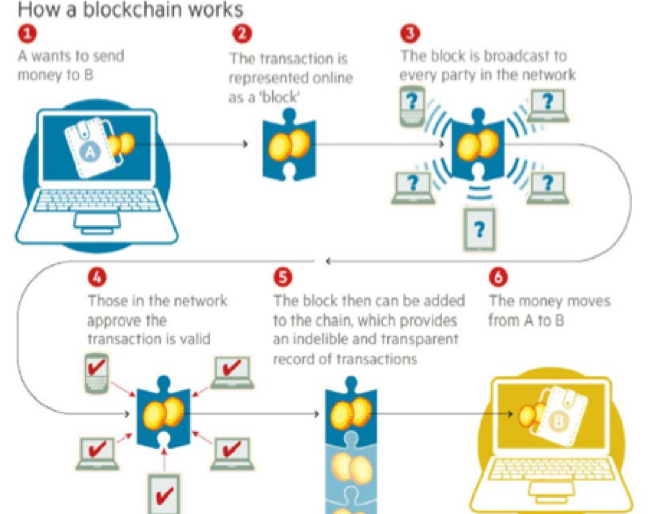
\includegraphics[width=\paperwidth-200pt]{images/blockchain?}
        \caption{Illustreert hoe de blockchain werkt \cite{howBlockchainWorks}}
        \label{fig:blockchain?}
    \end{center}
\end{figure}
\newpage

In dit onderzoek gebruiken we de beschrijving van het ICTU \footnote{https://www.ictu.nl/}, die de blockchain beschrijft als: een specifieke databasetechnologie die leidt tot een gedistribueerd autonoom grootboeksysteem \cite{kaptijn}. De integriteit van dit gedistribueerd autonoom grootboeksysteem wordt gewaarborgd doordat iedere partij zeggenschap heeft bij de validatie van een transactie. Dit versnelt het proces doordat beheerders en tussenpersonen worden uitgeschakeld. Meningsverschillen worden opgelost door een cryptografisch consensus algoritme (zie paragraaf \ref{cap:consensus}).\par

De blockchain technologie lost verschillende problemen op die voorkomen bij het gebruik van traditionele gecentraliseerde database technologieën die in handen zijn van één instantie. Dit soort technologieën vereisen vertrouwen dat de beheerder zorgvuldig omgaat met de toegang of bewerkingen van de data. Verder dient de database toegankelijk te zijn voor de belanghebbende en dat hij erop kan vertrouwen dat de instantie er de volgende dag nog is. Deze problemen komen niet voor in een gedecentraliseerde blockchain database. Dit komt omdat een nieuwe dienst, softwarebedrijf of markten op de blockchain de volgende zes designprincipes \cite{blockRev} hanteren:
\begin{enumerate}
	\item Netwerk integriteit\\
	Het systeem bewaakt de data integriteit doordat ieder lid in het netwerk alle transacties kan nalopen en kan controleren, in plaats van een enkel lid die dit proces uitvoert. Gebruikers op het netwerk kunnen rechtstreeks waarde met elkaar uitwisselen door dit te registeren op een blok. Elk blok heeft een verwijzing naar een voorgaand blok, waardoor niemand een transactie kan verbergen of kan vervalsen. Dit omdat er meer andere gebruikers zijn met de juiste realiteit.
	\item Gedistribueerd\\
	Het systeem is volledig Gedistribueerd. Dit houdt in dat er geen één punt is van controle of falen. Er is niet een gebruiker of organisatie die het systeem uit kan zetten.
	\item Security\\
	Satoshi’s white paper \cite{bitcoinPaper} vereist dat het systeem beveiligd is door een public key infrastructure (PKI) \footnote{https://en.wikipedia.org/wiki/Public\_key\_infrastructure}. De PKI is een geavanceerde vorm van asymmetrische cryptografie, waar de gebruiker zowel een publiek en privé sleutel ontvangt om zichzelf binnen het netwerk te identificeren en berichten kan versleutelen en ontsleutelen.
	\item Eigendomsrechten\\
	Eigendomsrechten over valuta en andere data zijn transparant in het netwerk en dus beschikbaar voor iedere gebruiker van het netwerk. Hierdoor dient een blockchain als een publiek register door middel van een tool genaamd Proof of Existence (PoE) \footnote{https://en.wikipedia.org/wiki/Proof\_of\_Existence}. Deze tool creëert en registreert de cryptografische overzichten van akten, licenties en andere rechten van gebruikers.
	\item Privacy\\
	Gebruikers beheren hun eigen data. Er is geen centrale partij en gebruikers op het netwerk geven zelf aan wat ze aan informatie vrijgeven. Dit is echter allemaal optioneel en een gebruiker op de blockchain hoeft in de meeste implementaties alleen een publieke en private key te hebben. De gehele identificatie- en verificatie laag zijn los van elkaar waardoor gebruikers op de blockchain de mogelijkheid hebben om anoniem te zijn.
	\item Valuta als motivatie\\
	Het systeem motiveert deelnemers van het netwerk door ze valuta te geven voor bepaalde acties op het netwerk. In het geval van de bitcoin, krijgen miners bitcoin geld voor het eerstvolgende blok te koppelen aan het vorige blok aan data. Dit wordt gedaan door een cryptografische puzzel op te lossen die geleidelijk lastiger wordt.
\end{enumerate}
\newpage

\section{Type Blockchain}
Om een geïnformeerd besluit te maken welk type blockchain juist is voor het proof of concept worden de verschillende type blockchain in dit paragraaf behandeld. Dit wordt gedaan vanaf een hoog technisch niveau. In essentie zijn er drie types blockchain: privé, consortium en openbaar. Deze types kunnen daarna weer onderverdeeld worden in de open en gesloten categorieeën blockchain. Per type blockchain wordt er ook gelijk gekeken naar de grote projecten die relevant zijn. Zodat in een vervolg hoofdstuk hierover een vergelijking kan worden uitgevoerd.\par
					
De categorie gesloten, waarin de types privé en consortium zitten zijn bedoeld voor een gelimiteerde omgeving zoals één of meerdere bedrijven en organisaties. Terwijl een openbare blockchain volledig open is en geen permissies zijn die mensen of systemen erbuiten houden.

\subsection{Privé Blockchain}
Voor een volledige private blockchain, moeten de schrijfrechten op een centrale plek staan die beheerd worden door een organisatie. De leesrechten kunnen zowel publiekelijk of ook net zo beperkt zijn als de schrijfrechten. Applicaties die gebruik maken van een privé Blockchain zijn interne applicaties die alleen gebruikt worden binnen een bedrijf of organisatie. Want in andere gevallen wordt publieke leesrechten en controleerbaarheid vereist \cite{privateBlockChains}. Voorbeelden van privé Blockchains zijn MultiChain en Hyperledger:\par
\textbf{MultiChain} - MultiChain is een platform voor het ontwikkelen en publiceren van privé blockchains. Het lost een aantal schaalbaarheid problemen \cite{oreillyScalability} van de blockchain op met een geïntegreerde gebruiker permissie systeem. Verder biedt het bedrijven de mogelijkheid om zonder software ontwikkelaars een blockchain op te richten \cite{mutlichain}.

\textbf{Hyperledger} - Hyperledger is een open source project. Het wordt ontwikkeld met als doel om een geavanceerd bedrijfstak overkoepelende blockchain implementatie te realiseren. Het wordt ondersteund door de Linux Foundation \cite{linuxFoundation} en wordt gezamenlijk ontwikkeld door grote organisatie in financiën, banken, IoT, productie en technologie \cite{hyperledger}.

\subsection{Consortium Blockchain}
Het consortium blockchain type is gedeeltelijk privé. Het onderscheidt zich in het consensus (zie paragraaf \ref{cap:consensus}) proces waar alleen een aantal vooraf geselecteerde peers (gebruikers) de integriteit van de data op de blockchain waarborgen. Deze nodes zijn bijvoorbeeld 10 grote financiële instellingen die bij de aanmaak van een nieuwe block aan de blockchain zeggenschap hebben. Andere deelnemers van de blockchain hebben nog steeds het recht om de besluiten van de 10 nodes te controleren, maar ze hebben verder geen stem over het feit of de volgende block valide is.\par
\newpage					
Het voordeel van de consortium variant is dat deze efficiënter is en toch voldoende transactie transparantie geeft. Ook is het niet een bedrijf die alleen oordeelt over de data. Voorbeelden van dit type zijn Ethereum en R3:

\textbf{Ethereum} - Het Ethereum project beschrijft zichzelf als een gecentraliseerd platform voor applicaties die precies uitgevoerd worden zoals ze geprogrammeerd zijn. Dit allemaal zonder enige kans van fraude, censuur of veranderingen van derden \footnote{https://www.ethereum.org/}. Applicaties, smart contracts, worden geprogrammeerd in de Solidity taal die voor het Ethereum project is ontwikkeld. Het wordt open-source ontwikkeld en er is een bondgenootschap, de Enterprise Ethereum Alliance\footnote{https://entethalliance.org/} dat bestaat uit 315 fortune 500 bedrijven en organisaties, die gezamenlijk werken aan het het enige platform die smart contracts ondersteunt op de blockchain.\cite{ethWood}\par

Het project kan gezien worden als een verder uitgewerkte versie van Bitcoin die meer functionaliteiten toevoegt. Zo bestaat de status van Ethereum netwerk net zoals de Bitcoin uit meerdere objecten die 'accounts' worden genoemd, waarbij elk account een adres van 20 bytes en statusovergangen heeft. De staat van deze objecten worden opgeslagen in de blockchain waaruit gelijk afgeleid kan worden waar valuta naartoe gaat.\cite{whitePaperEthereum}

\textbf{R3} - Dit is een gedistribueerd database-technologiebedrijf in New York. Het is verbonden met veel van ’s werelds grootste financiële instellingen, met als missie om de voordelen van de blockchain te realiseren. Het is momenteel nog enorm in ontwikkeling en het bedrijf voert vooral onderzoek uit\cite{R3}.

\subsection{Openbare Blockchain}
Dit type blockchain is zoals de naam al aangeeft publiek beschikbaar tot iedereen in de wereld. Dit houdt in tegenstelling tot Consortium ook het consensus (zie paragraaf \ref{cap:consensus}) proces in. Iedere gebruiker op het netwerk is gelijk en heeft zeggenschap op de geldigheid van nieuwe data blokken.\par

Een volledig publieke blockchain is een open-source systeem die gebruikers met economisch doeleinde motiveert om samen te werken. Dit principe heet crypto economics en hierdoor kunnen ontwikkelaars belangen zoals beschikbaarheid waarborgen. Zo zal een transactie met een hoger tarief resulteren in snellere conversie. Een voorbeeld hiervan is het bekende Bitcoin project.

\textbf{Bitcoin}. Bitcoin is het bekendste voorbeeld van een blockchain project. Bitcoin staat vooral bekend als digitale valuta en online betalingssysteem die door gebruik van cryptografie om valuta-eenheden te geneert en reguleert. Verder gebruikt het cryptografie om de overdracht van fondsen te verifiëren zonder een centrale bank.\par
\chapter{De architectuur van de blockchain technologie}
Dit hoofdstuk gaat iets verder in op de basis architectuur van de blockchain. Dit zodat tijdens het ontwikkelen van de Proof of Concept we de basis begrippen van de architectuur begrijpen.

\section{Blok (block)}
De blockchain bied een gedistribueerd grootboeksysteem. Gegevens worden permanent opgeslagen in het netwerk via bestanden die blokken worden genoemd. Een blok is een document alle recente transacties die nog moeten worden vastgelegd. Het heeft daarom de naam blockchain, omdat het een reeks van blokken die naar de vorige verwijzen\cite{blochchainTechSymmbioticDev}.\par

Een blok in het geval van de Bitcoin bestaat uit een header en een body \cite{blockchainIssuesAndChallenges}. De header bestaat uit drie stukken meta gegevens. De eerste is een verwijzing naar een vorige blokhash (Merkle-hash\footenote{https://en.wikipedia.org/wiki/Merkle_tree}). Hierdoor verbindt het blok met de vorige uit de blockchain. De tweede set van meta gegevens is  moelijkheidsgraad, tijdstempel en nonce. Het laatste stuk metadata is de Merkle-tree root, een datastructuur die wordt gebruikt om alle transacties in het blok efficiënt samen te vatten \cite{masteringBitcoin}.

\section{Gedecentraliseerd netwerk}
The interactions among user on blockchain principally use a decentralized network in which each user represents a node at which a blockchain client is installed. When a user performing a transaction with another user or when a node receives data from another node, it verifies the authenticity of the data. It then broadcasts the validated data to every other node connected to it [86]. Within such a mechanism, the data spreads across the whole network. The benefit of using this mechanism is the centralization of the human factor is minimized and trust shifts from the human agents of a central organization to an open source code [5].
\newpage

\section{Consensus (overeenstemming) algoritmes}
Om de werking van de blockchain te begrijpen en te vertrouwen, moet het begrip van Consensus oftewel overeenstemmings algoritmes duidelijk zijn. Deze algoritmes worden gebruikt wanneer een (nieuw) blok aan informatie geverifieerd wordt. Het zorgt voor één historie van transacties waar de geschiedenis geen ongeldige of tegenstrijdige transacties bevat.\par

Dit is allemaal nodig omdat de blockchain draait in een zelf gereguleerde, wantrouwende omgeving waar het nodig is om meningsverschillen over transacties binnen het netwerk op een lijn te krijgen. Het zorgt er bijvoorbeeld ook voor dat er niet één account is die meer uitgeeft dan dat het heeft, of waar hij of zij twee keer iets overmaakt, dit heet double-spending. De bekende consensus algoritmes zijn proof of work en proof of stake.\par

\begin{enumerate}
	\item Proof of Work (PoW)\\
	Het PoW consensus algoritme is het meest voorkomende algoritme in blockchain. Het werd geïntroduceerd door de Bitcoin en gaat ervan uit dat alle peers met rekenkracht mee stemmen door PoW-instanties, crytografische puzzels op te lossen en hiermee het recht hebben om de volgende blok aan te maken in het netwerk. Zo maakt de Bitcoin gebruik van een hash-gebaseerde PoW, wat inhoudt dat de peers een nonce-waarde \footnote{https://en.wikipedia.org/wiki/Cryptographic_nonce} proberen te vinden. Hierbij is wel de voorwaarden dat de vorige blokhash kleiner moet zijn dan de huidige doelwaarde die in de blokparameters staat van het vorige blok. Wanneer een dergelijke nonce wordt gevonden, maakt de miner het blok aan en stuurt hij het door naar zijn peers. Deze peers ontvangen dit dan en verifiëren of het klopt aan de hand van het vorige blok \cite{securityPOW}.
	\item Proof-of-Stake (PoS)\\
	Op het moment moet Proof-of-Stake zich nog bewijzen in de crypto valuta gemeenschap. Het is ontwikkeld om bestaande inefficiënte consensus algoritmes zoals PoW te vervangen. Het algemeen begrip van PoS is dat een peer (deelnemer van de blockchain), pas het stemrecht heeft op een nieuwe blok in de blockchain als de peer voldoende heeft ingezet in het netwerk. In het geval van PeerCoin \footnote{https://peercoin.net/} worden nieuwe blokken gegeneerd door het netwerk op basis van niet gespendeerde valuta en hoe oud deze is \cite{posProtocol}.\par
	
	Met deze methode wordt aangenomen dat mensen met meer valuta minder snel het netwerk zullen aanvallen \cite{blockchainIssuesAndChallenges}. Dit lost op het gebied van energiebesparing de problemen van PoW op, waar gebruikers miners aan zetten om valuta te ontvangen. Bij PoS wordt de valuta die niet beweegt steeds meer waard.
\end{enumerate}

\section{Smart contract}
Het idee achter smart contracts is een "geautomatiseerd transactieprotocol dat de voorwaarden van een contract uitvoert" \cite{smartContracts} en werd voor het eerst bedacht door cryptograaf Nick Szabo. Dit idee is door de opkomst van de blockchain populair geworden. Dit komt door dat de blockchain gedecentraliseerd is en daardoor de tussenpersonen bij een gecentraliseerde smart contracts applicatie eruithaald. Smart contracts is, in de context van blockchain, gewoon software die op een blockchain wordt gepubliceerd en die transacties kan ontvangen of uitvoeren. Iedere transactie heeft een adres en kan worden gevolgd. \par
\chapter{Conclusie}\label{chap:conclusion}
Het type privé blockchain kan voor het proof of concept direct uitgesloten worden. Dit omdat het hele idee van het proof of concept gaat om het feit dat alle transacties transparant zijn voor alle deelnemers van het netwerk. Zodat bijvoorbeeld verzekeraars een transactie kunnen verifiëren voordat ze hem uitbetalen.\par

Hierna houden we alleen nog het Consortium en openbaar type blockchain over. Hierbij is gekozen voor consortium omdat deze efficiënter is in het verwerken van transacties. Daarnaast zit in de consortium variant het project Ethereum, die momenteel de enige is die smart contracts biedt op de blockchain.\par

Verder is de conclusie dat de technologie om de blockchain en hoe deze werken nu duidelijk en kan er ontwikkeld worden aan het proof of concept.

%%%%%%%%%%%%%%%%%%%%%%%%%%%%%%%%%%%%%%%%%%%%%%%%%%%%%%%%%%%%%%%%%%%%%%%%%%%%%%
%%
%% Bibliography:
%%
%\cleardoublepage
%\phantomsection
\addcontentsline{toc}{chapter}{Bibliografie}
\bibliography{thesis}

% %%%%%%%%%%%%%%%%%%%%%%%%%%%%%%%%%%%%%%%%%%%%%%%%%%%%%%%%%%%%%%%%%%%%%%%%%%%%%%%%
% %% Appendix:
% %%

%\chapter{Bijlagen}

\end{lstlisting}


%%%%%%%%%%%%%%%%%%%%%%%%%%%%%%%%%%%%%%%%%%%%%%%%%%%%%%%%%%%%%%%%%%%%%%%%%%%%%%%%
%% Index:
%%
% \printthesisindex

\end{document}
